\section{Inverted Pendulum Hardware}
The following section describes the hardware connected to the inverted pendulum setup illustrated cf. figure \ref{fig:InvertedPendulumSetUp}.
Each part will be described with its specifications and use in the setup.

\subsubsection{Stick and Arm}
The arm and stick is elements that always appears in the double inverted pendulum setup. The goal is for the arm to apply force on their common joint, which would affect the position of the stick. The physical parameters for the stick and arm is listed cf. table \ref{DimensionsStick}.

\begin{table}[htbp]
\centering
\begin{tabular}{llll}
\hline
Piece           & Parameter & Value & Unit \\ \hline
Stick$_{long}$  & Length    & 0.8   & [m]    \\
Stick$_{long}$  & Weight    & 0.344 & [kg]    \\ \hline
Stick$_{short}$ & Length    & 0.4   & [m]    \\
Stick$_{short}$ & Weight    & 0.170 & [kg]    \\ \hline
Arm             & Length    & 0.33  & [m]    \\
Arm             & Weight    & 288   & [kg]   \\ \hline
\end{tabular}
\caption{Physical parameters of the arm and sticks.}
\label{DimensionsStick}
\end{table}

Some feedback is needed to be able to control the stick trough the arm and gears. Sensors used is implemented as a integrated part of the setup, and will therefore be considered usable and will the choice of the will not be further discussed.

A necessary feedback is the angle between the stick and arm, to know if control is needed to balance the stick. The angle between the stick and arm is detected and sampled via a potentiometer. Equally the position of the arm is needed, this is to determine the amount of change needed to counteract the change in the stick. The position of each potentiometer can be seen cf. figure \ref{fig:InvertedPendulumSetUpPotmeter}. 

\begin{figure} [htbp]
	\centering
	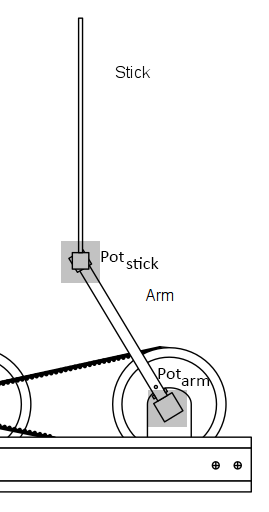
\includegraphics[width=0.35\linewidth]{figures/"Preanalysis&Requirement"/invertedPendulumWithPotmeter.PNG}
	\caption{Diagram of the arm and stick with illustrated sensors.} \label{fig:InvertedPendulumSetUpPotmeter}
\end{figure}
\newline


\subsubsection{DC Motor}
Alsthom BBC MODEL: F9M2 AAU:08339
\ref{appendix:DCMotorInductance}

The third feedback implemented is the velocity of the motor. The motor given  

\subsubsection{Gear System}
Gear teeth big: 40
Gear teeth small: 12
Belt length: 60 cm
Wheel diameter big: 12 cm
Wheel diameter small: 4 cm

